\documentclass[tikz,border=1pt]{standalone}
\usetikzlibrary{positioning}
\begin{document}

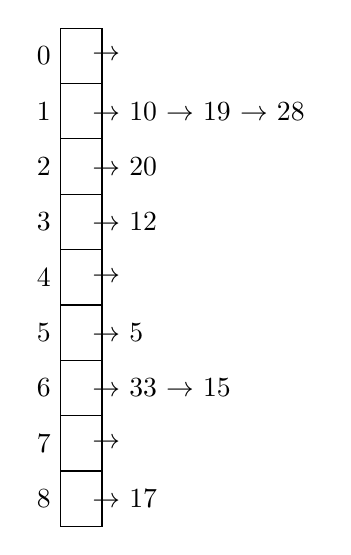
\begin{tikzpicture}
\coordinate (0);
\foreach \t[count=\i from 0,evaluate=\i as\j using int(\i+1)] in {
 ,
 10 $\rightarrow$ 19 $\rightarrow$ 28 , 
 20 ,
 12 ,
 ,
  5 ,
 33  $\rightarrow$ 15 ,
 ,
 17
}
\node at(\i.south)[anchor=north,draw,minimum height=2em,minimum width=1.5em,outer sep=0pt](\j){}
    node at(\j.west)[align=right,left]{\i}
    node at(\j.east)[align=left,right,xshift=-.7em]{$\rightarrow$ \t};
\end{tikzpicture}

\end{document}